%----------------------------------------------------------------
%
%  File    :  available_dataset.tex
%
%  Authors : Thomas Lerchbaumer
% 
%  Created :  19 March 2022
% 
%  Changed :  19 March 2022
% 
%----------------------------------------------------------------

\chapter{Available Dataset}
\label{chap:available_dataset}
This chapter focuses on explaining and analysing the available data. The data is analyzed for Business Intelligence (BI) purposes as well as on metrics that can be used to create predictions. Whereas BI \cite{9325610} focuses on historical data and aims to support managers to make decisions traditional methods like predictive analytic asses potential future scenarios using advanced statistical methods \cite{9671997}.

\section{Data Origin}
The available dataset is gathered from a website that provides a service to find and book buses for individual journeys. This service is currently available in Austria, Germany, Switzerland and Lichtenstein. The buses itself are offered in real time by various different bus companies. Offers can vary in price which is based bus calculations which may vary from operator to operator. The data is stored in a relational database. Since the service also provides the possibility to directly book a bus, booking and corresponding user meta data is available as well. \newline




\section{Data Structure}
The service launched in March 2017 therefore booking data is available back to this date. Tracking the search requests was introduced in October 2020. 
The request table itself keeps track of 40 attributes but not all of them host valuable information that could be analysed therefore only the ones which can be analysed are listed and explained below:

\begin{itemize}
  \item \verb|task_id| - PK (incremented value) 
  \item \verb|createdAt| - At which time the search request was made.
  \item \verb|accountId| - Not empty when the user is currently logged in
  \item \verb|amountSearchResults| - How many buses can be offered
  \item \verb|containsTripCompany| - If the user wants to stop at a certain company during the trip
  \item \verb|distanceInMeters|  - Distance between departure and destination place
  \item \verb|durationInSeconds| - Duration of the trip
  \item \verb|pax|  - Amount of passengers
  \item \verb|taskFrom_address| - Departure address 
  \item \verb|taskFrom_lat and lng| - Latitude and Longitude of the departure
  \item \verb|taskTo_address|  - Destination address
  \item \verb|taskTo_lat and lng| - Latitude and Longitude of the destination
  \item \verb|taskFrom_Time|  - Desired departure time 
  \item \verb|taskTo_Time|  - Estimated arrival time
  \item \verb|cheapestPrice_amount| - The cheapest price for a bus
  \item \verb|bus_id| - The operator with the cheapest bus
  \item \verb|city| - From which city the request was made
  \item \verb|country| - From which country the request was made
\end{itemize}

Whenever a booking is made the correlating data is stored within a booking table. As the booking table contains sensitive data which is not scope of the analysis, so only three attributes are used: 

\begin{itemize}
	\item \verb|createdAt| - At which time the booking was made.
	\item \verb|company_id| - FK used to identify who received the booking
	\item \verb|task_id| - FK used to link the booking to an search request 
\end{itemize} 

\section{Data Cleansing}
\label{sec:data_cleansing}
During this process the available data is investigated for irregularities that cause distortion when applying statistical models. 

Search requests are tracked whenever a user opens the service and searches for a certain connection. Given that behaviour it may occur that a user searches for the same connection within a short time window. This behaviour results in the need of de-duplication to avoid bias. To filter out duplicates the attributes \verb|ipHash|, \verb|createdAt|, \verb|taskFrom_address| and \verb|taskTo_address|. A search request is considered as non duplicate whenever the timespan between equal entries is larger than one hour. 
To pre-process the data the following logic is applied once //todoChange: 
\begin{lstlisting}
    query = '''
    DELETE t1
    FROM search_requests_clean t1
    INNER JOIN search_requests_clean t2
        ON t1.taskFrom_address = t2.taskFrom_address
        AND t1.taskTo_address = t2.taskTo_address
        AND t1.ipHash = t2.ipHash
        AND t1.createdAt > t2.createdAt
        AND t1.createdAt - t2.createdAt <= %s
	'''

    timespan = 3600  # 3600 seconds  - 1 hour
    cursor = connection.cursor()
    cursor.execute(query, (timeframe,))
    connection.commit()
\end{lstlisting}

//todo more explanation
The logic above compares all entries based on the attributes mentioned above removes equal entries that are within a timespan of 1 hour. 

Regarding validation and norming the available data present in both tables no actions are required due to fact that attributes that do not meet their defined data types are not stored in first place. 

\section{Data Augmentation}
\label{sec:data_aug}
Starting from March 2020 countries like Austria, Germany, Switzerland and Lichtenstein had to put travel restrictions into effect due to the ongoing Covid19 pandemic \\citeHere. This travel restrictions impacted the gathered booking data as those restrictions forbid travelling.
\begin{figure}[H]
	\centering
		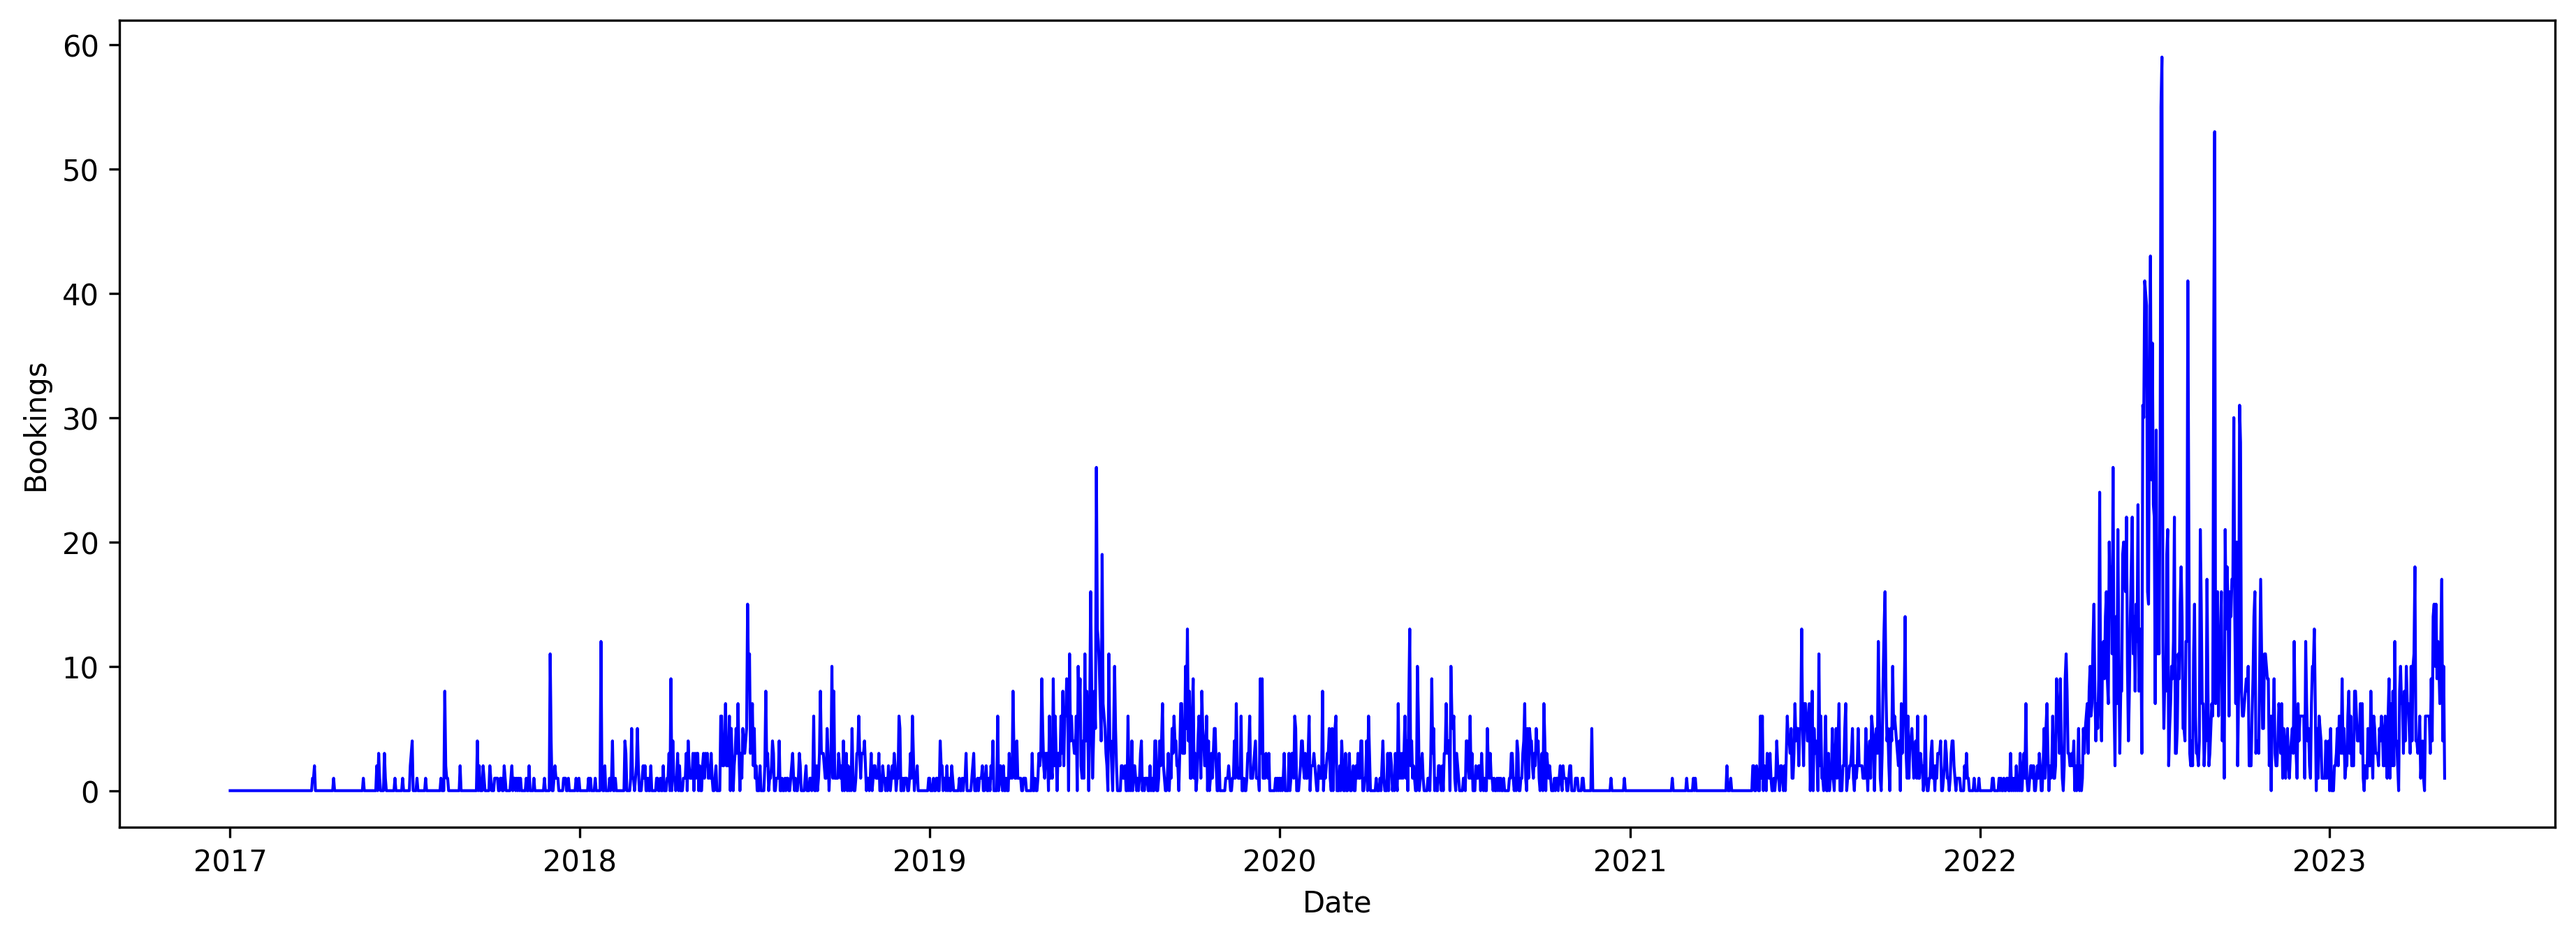
\includegraphics[width=14cm]{images/no_augmentation}
	\caption{Bookings over time - [source:author]}
	\label{fig:noAug}
\end{figure}
Figure \ref{fig:noAug} highlights the drop of bookings starting from March 2020 until June 2022. To achieve reliable results when utilizing this data for a time series forecasting ML model this time period needs augmentation. When analysing the chart \ref{fig:noAug} an continuous growth of bookings is visible until 2021. One way to augment the data \\citehere is calculate the average growth during this time span. To substitute the distorted data the current data is replaced by the value of the previous year. This value is then multiplied by the average growth. Furthermore missing timestamps throughout the whole time series are added with a value of zero. The following logic is applied to the data frame: 

\begin{lstlisting}
df = db.get_booking_data()
average_growth = df['bookings'].pct_change().mean()
substitute_corona = pd.date_range(start='2020-03-01', end='2022-05-01', freq='D')
df['date(createdAt)'] = pd.to_datetime(df['date(createdAt)'])
df = (df.set_index('date(createdAt)')
      .reindex(pd.date_range('2018-01-01', '2023-05-01', freq='D'))
      .rename_axis(['date(createdAt)'])
      .fillna(0)
      .reset_index())

df.set_index('date(createdAt)', inplace=True)

for date in substitute_corona:
    year_ago = str(date - relativedelta(years=1)).split(" ")[0]
    val = int(math.ceil(df.loc[year_ago]['bookings'] * (1+average_growth)))
    df.loc[str(date).split(" ")[0]] = val
\end{lstlisting}

The average growth per anno is around 30\%. After applying the logic the data set looks the following:  
\begin{figure}[H]
	\centering
		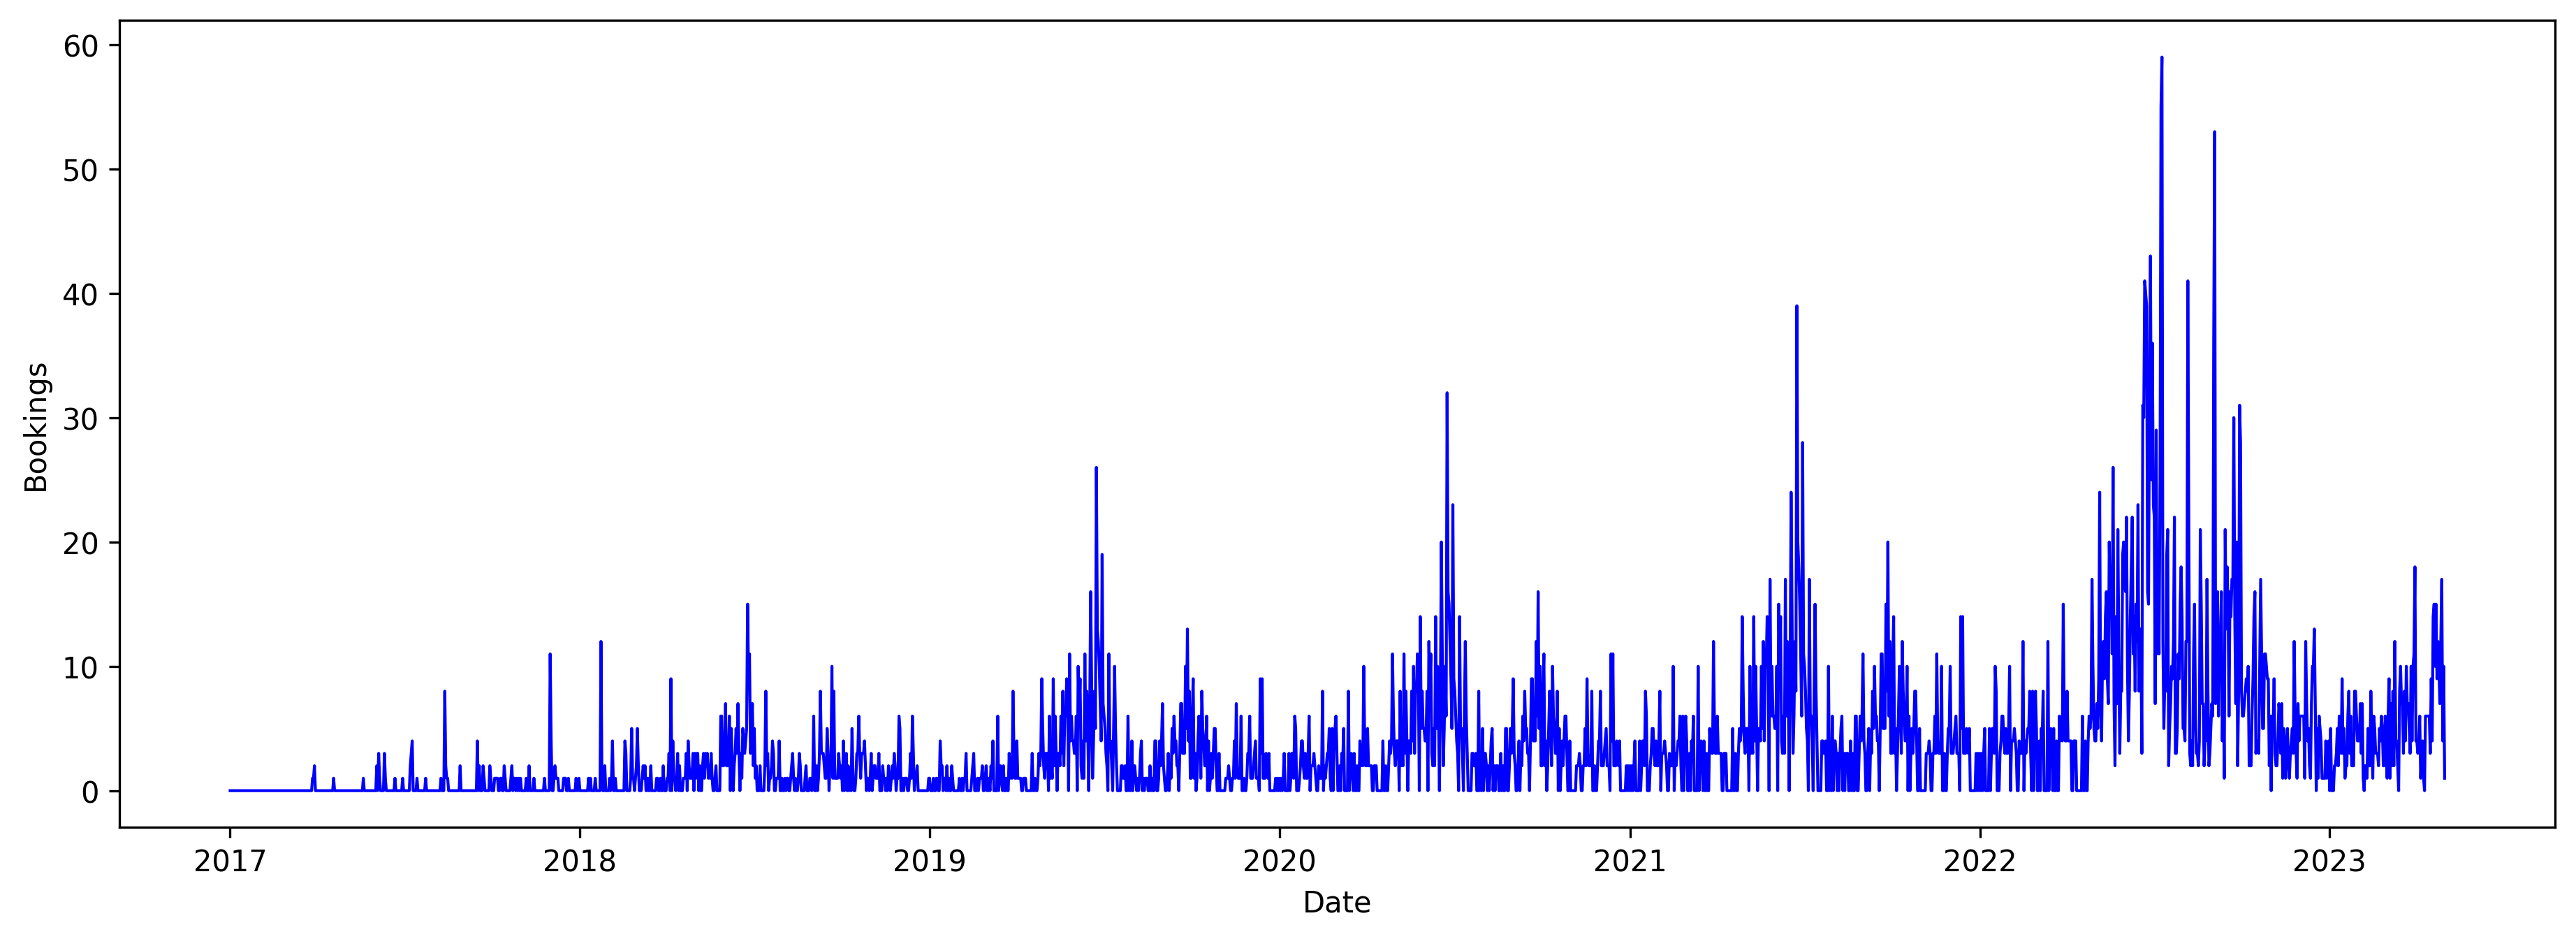
\includegraphics[width=14cm]{images/with_augmentation}
	\caption{Augmented Data Set - [source:author]}
	\label{fig:noAug}
\end{figure}
The impact of this augmentation in terms of prediction accuracy is compared in chapter \ref{chap:prediction_model}.

\section{What insights can be gathered?}
This section focuses on which potential information from the available dataset can be extracted and utilized for a reporting dashboard. Furthermore the dataset will be analysed for metrics that can support and improve the current yield management. 


\subsection{Improving the Yield Management}
In general Yield Management (YM) describes the way how limited resources like hotel rooms, seats within an air plane or available buses are assigned to customers by levearging the highest possible revenue. American Airlines claims that by utilizing YM they are able to increase their revenue by 500 million dollars per year \cite{ym_practice}. Before integrating YM a few considerations about the characteristics of teh provided service need to be made otherwise YM might actually cause a decrease in revenue. The following characteristics are suitable for the utilization of YM:\cite{ym_practice}
\begin{itemize}
  \item Storing surplus resources can either be costly or unattainable. 
  \item Whenever future demand is uncertain commitments need to be done.
  \item It is possible to differentiate between customer segments
  \item A single unit can be used to provide different services 
  \item The company is not legally limited in their actions of selling a certain service or not.
\end{itemize}
As YM is already in place at busfinder one of the characteristics mentioned above comes along with a high uncertainty. Although commitments for uncertain future demand are made the ability to predict future bookings would further improve the YM. Being able to predict future bookings during ordinary market conditions (e.g. no travel restrictions in place) those estimates directly can be used to influence factor of capacity management - How many buses are available? This directly influences the pricing strategy because a higher demand results in a higher price.

Both Artificial Neural Networks (ANNs) and their usage for time series forecasting further evolved over the past years. Additionally libraries like tensorflow  reduce the complexity of developing ANNs. Hence this method is a suitable solution to predict future bookings. Therefore the basics of ANN and the development of two different models are explained in chapter \ref{chap:predict}.


